\section{Dataset scelto}

Il dataset scelto per il nostro scopo è \href{https://huggingface.co/datasets/kili-technology/plastic_in_river}{kili-technology/plastic\_in\_river}
che raccoglie immagini di laghetti e bacini d'acqua con oggetti e/o rifiuti in superficie. 
Il dataset è stato creato per la \href{https://kili-technology.com/data-labeling/machine-learning/kili-s-community-challenge-plastic-in-river-dataset}{Kili's Community Challenge},
sfida nata per invogliare la community di sviluppatori a sfruttare i modelli di deep learning per contrastare il problema dell'inquinamento degli oceani. 
La sfida si è svolta nel febbraio 2022 e il dataset è rimasto accessibile pubblicamente anche dopo la fine 
dell'evento\footnote[1]{Attualmente (luglio-agosto 2024) si riscontrano \href{https://huggingface.co/datasets/kili-technology/plastic_in_river/discussions/2}{problemi} nell'acquisizione del dataset tramite API. Probabilmente il proprietario del dataset 
ha spostato o tolto il dataset dal proprio server. Per il momento non si sa se il dataset tornerà a disposizione senza problemi}. 

Il dataset è composto da un totale di 4259 immagini, già divisi in tre sottoinsiemi per training, validazione e test. Nella tabella \ref{table:1} 
è possibile vedere la ripartizione delle istanze per sottoinsieme. Ogni immagine ha anche un file di testo con 
la lista degli oggetti presenti all'interno, classe dell'oggetto e posizione spaziale rispettando il data format usato da YOLO.

\begin{table}[h!]
    \centering
    \begin{tabular}{ |c||c| } 
     \hline
     \textbf{Subset} & \textbf{Numero istanze} \\ 
     \hline
     Train & 3407 \\ 
     Val & 425 \\ 
     Test & 427 \\ 
     \hline
     Totale & 4259 \\
     \hline
    \end{tabular}
    \caption{Distribuzione delle immagini negli insiemi di train, val e test }
\label{table:1}
    \end{table}

Le categorie a disposizione per poter classificare gli oggetti identificati sono 4 e sono:

\begin{itemize}
    \item 0 : \verb+PLASTIC_BAG+
    \item 1 : \verb+PLASTIC_BOTTLE+
    \item 2 : \verb+OTHER_PLASTIC_WASTE+
    \item 3 : \verb+NOT_PLASTIC_WASTE+
\end{itemize}

La distribuzione delle classi tra le istanze non è uniforme ed è uno dei possibili problemi da affrontare durante l'addestramento del modello.
Il rischio è quello di avere difficoltà nel riconoscimento delle categorie che sono meno rappresentate all'interno del dataset.
Nella tabella \ref{table:2} è possibile vedere il numero di istanze per classe all'interno dei vari subsets.

\begin{table}[h!]
    \centering
    \begin{tabular}{ |c|c|c|c| } 
    \hline
    \textbf{Classe} & \textbf{Train} & \textbf{Val} & \textbf{Test} \\ 
    \hline
    \verb+PLASTIC_BAG+ & 1250 & 167 & 85 \\ 
    \verb+PLASTIC_BOTTLE+ & 6276 & 785 & 854 \\ 
    \verb+OTHER_PLASTIC_WASTE+ & 3345 & 296 & 122 \\ 
    \verb+NOT_PLASTIC_WASTE+ & 1414 & 212 & 111 \\
    \hline
    \end{tabular}
    \caption{Distribuzione delle istanze all'interno del dataset}
\label{table:2}
\end{table}

Le dimensioni delle immagini sono varie ma generalemente di qualità alta: la dimensione in larghezza supera i 1000 pixel e gli 800 pixel in altezza.

Nella immagine \ref{fig:1} è possibile in ordine vedere la distribuzione delle istanze nel dataset, la grandezza dei box per istanza all'interno dell'immagine, la distribuzione delle coordinate x e y del box nell'immagine, infine la grandezza del box per istanza.

\begin{figure}[h]
    \centering
    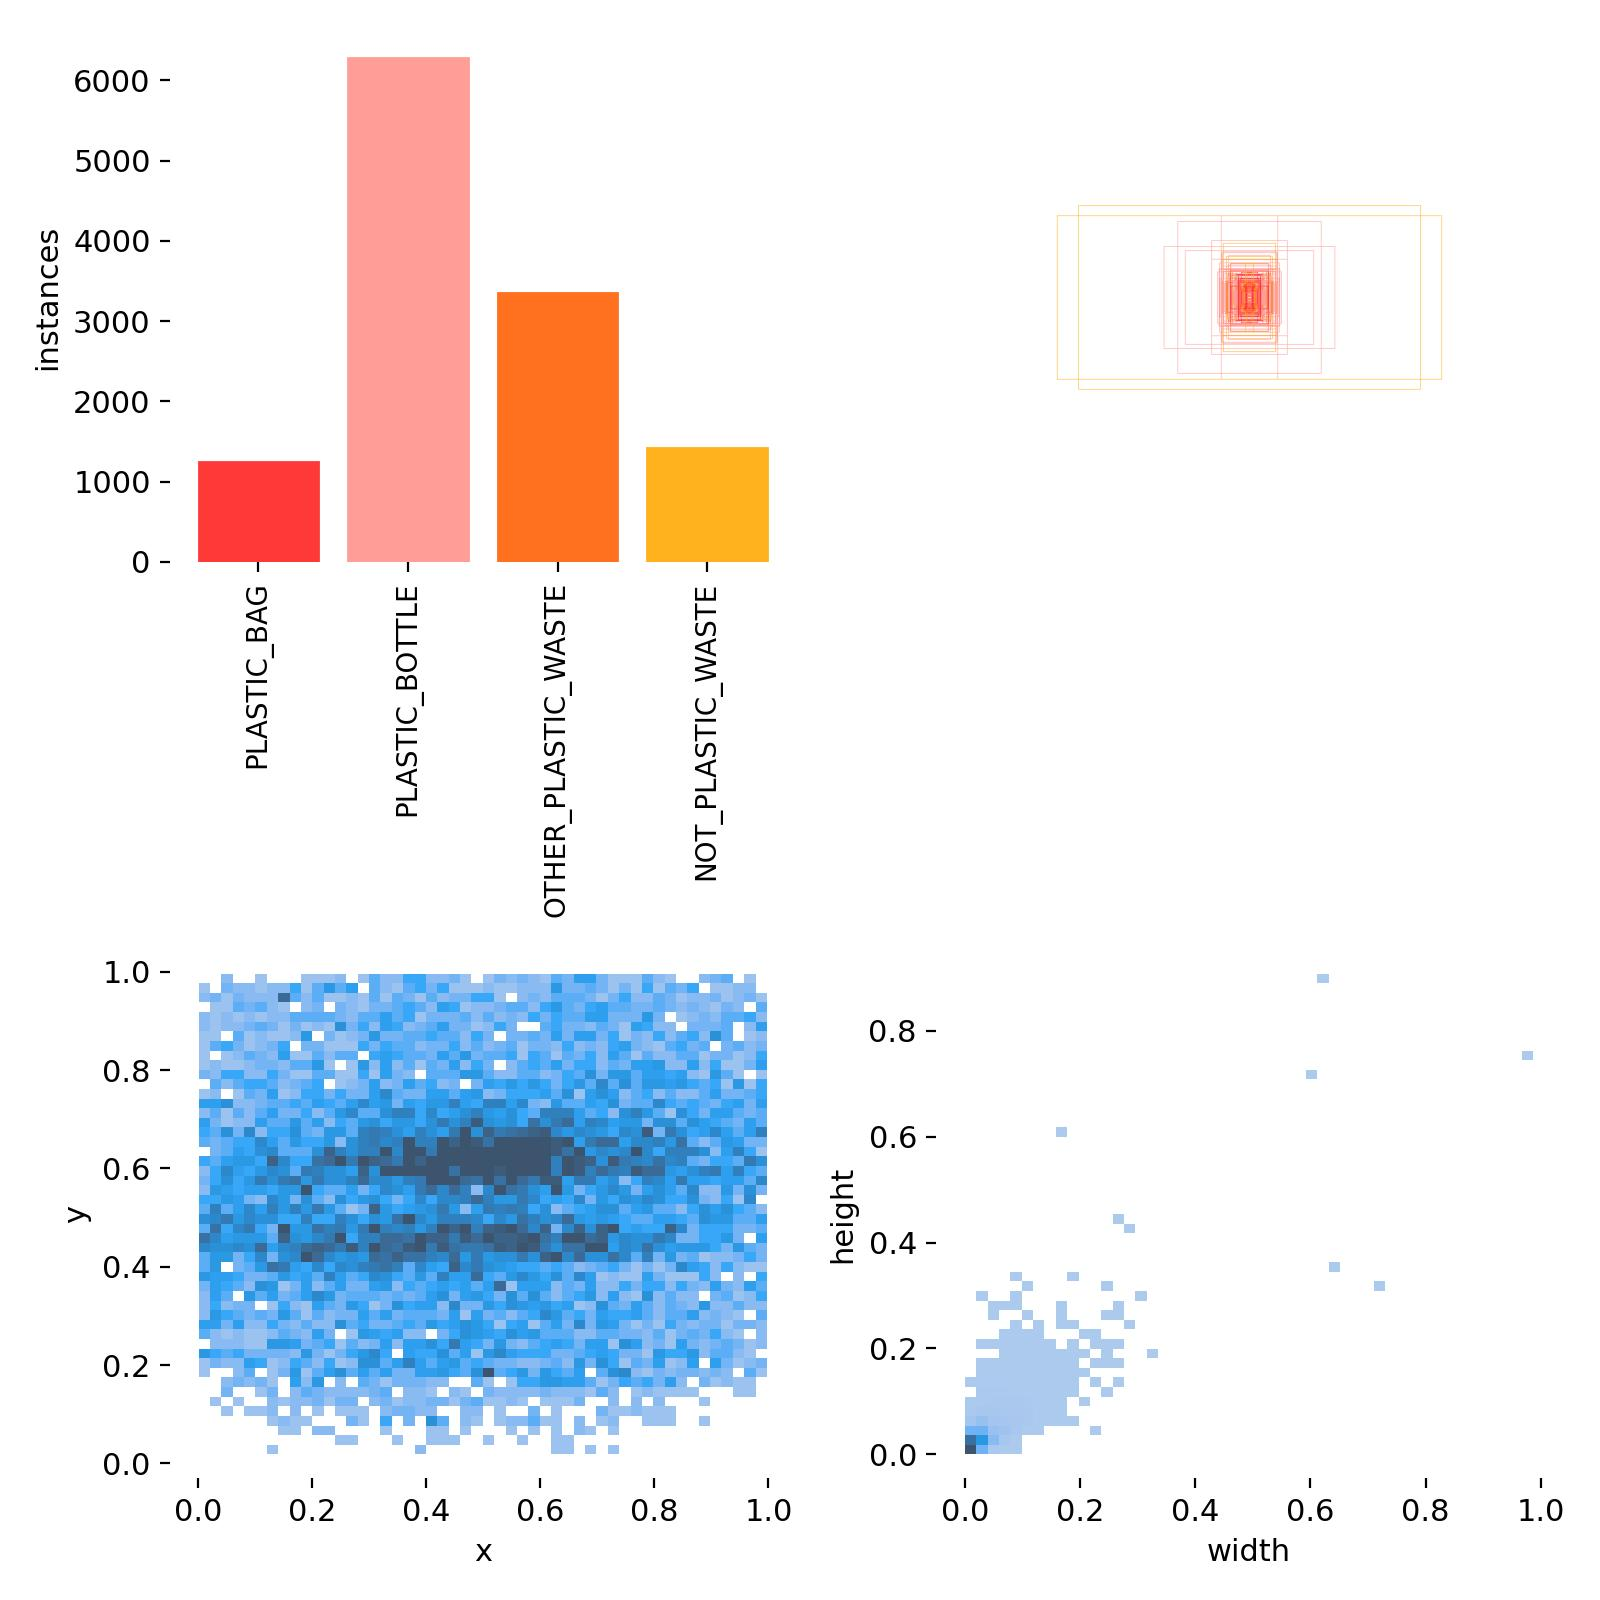
\includegraphics[width=0.8\textwidth]{labels.jpg}
    \caption{Caratteristiche istanze nel dataset}
    \label{fig:1}
    \end{figure}

Da notare come la maggior parte delle istanze hanno una dimensione della box rispetto all'immagine ridotta, in genere inferiore al 20\% della larghezza e/o altezza dell'immagine. In genere la maggior parte delle istanze, essendo rifiuti sulla superficie dell'acqua, sono concentrati orizzontalmente nella parte centrale dove è plausibile trovare l'orizzonte dello specchio idrico.

La dimensione ridotta del box potrebbe essere utile da tenere in considerazione per quanto riguarda l'iperparametro \verb+imgsz+, image size, ovvero le dimensioni delle immagini in ingresso passate al modello.